% 24th, Jan, 2001 Ver.1     Tatsuya Okabe
%                 Ver.2
%                 Ver.3
%                 Ver.4
%                 Ver.5
%
%---------------------------------------------------------------------------%
% Made by Tatsuya Okabe ( HONDA R&D Europe ( Deutschland ) GmbH )           %
% Checked by Bernhard Sendhoff ( HONDA R&D Europe ( Deutschland ) GmbH )    %
%---------------------------------------------------------------------------%
% Class LogNormal

\section{Abstract}

\noindent
With the class {\em LogNormal}, we can simulate the ``Log Normal''
distribution. If the logarithm $log(x)$ is normally or {\em Gaussian}
distributed, the distribution of {\em x} is called the {\em Log
Normal} distribution. The equation for this distribution is given below.

\begin{equation}
f(x) = \left\{
\begin{array}{ll}
\frac{1}{\sqrt{2\pi} \sigma x} \cdot \exp \left\{ \frac{-(\log x - \mu )^2}{2 \sigma^2} \right\} & x>0 \\
0 & x \le 0
\end{array}
\right.
\end{equation}

\noindent
In this equation, $x$, $\sigma$ and $\mu$ mean the variable, the
deviation and the average, respectively.

\vspace*{10mm}

\begin{center}
\begin{figure}[h]
\rotatebox{-90}{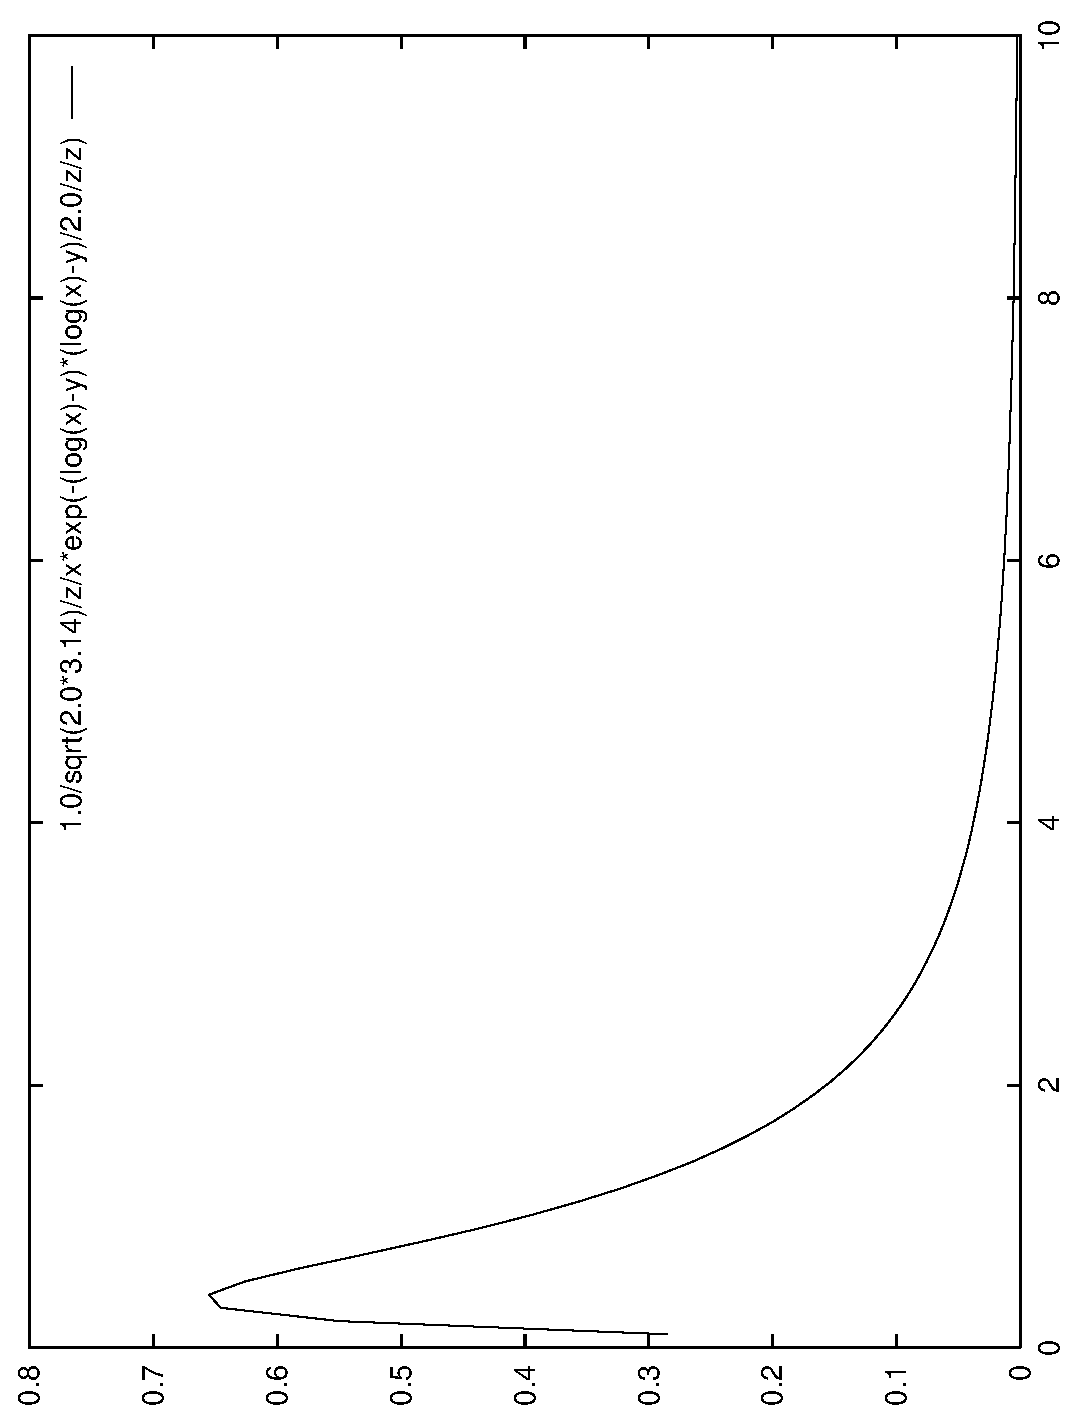
\includegraphics[height=12cm]{lognormal.eps}}\\
\caption{The Log Normal distribution. $\sigma=e(e-1)$ , $\mu=\sqrt{e}$.}
\end{figure}
\end{center}

\clearpage

\section{Internal Variables}

\begin{itemize}
\item logMean - The average.
\item logVariance - The variance.
\end{itemize}

%********************
\index{logMean (Variable)}
\index{logVariance (Variable)}
%********************

\vspace*{10mm}

\section{Public Methods}

\noindent
These methods can be used by all \cpp - programs, that have included the
header file LogNormal.h and the library EA. If you declare only
Population.h, we can't use these methods in this version.

\subsection{Constructors}

%---------------------------------------------------------------------------%
% 001
\index{LogNormal!( double mean, double variance )}
\setNormalInstance
\setCorrectWidthThree{8pt}
\setParamOne{mean}{double}{The average.} 
\setParamTwo{variance}{double}{The variance.}
\printMethodWithParamsSaved
{}
{None.}
{LogNormal}
{The default constructor. Generates the random generator of Log Normal
distribution.}
{None.}
\setCorrectWidthThree{4pt}
%---------------------------------------------------------------------------%

%---------------------------------------------------------------------------%
% 002
\index{LogNormal!( double mean, double variance, RNG\& rng )}
\setNormalInstance
\setCorrectWidthThree{8pt}
\setParamOne{mean}{double}{The average.} 
\setParamTwo{variance}{double}{The variance.}
\setParamThree{rng}{RNG\&}{RNG class.}
\printMethodWithParamsSaved
{}
{None..}
{LogNormal}
{The constructor. Generates the random generator of Log Normal distribution.}
{None.}
\setCorrectWidthThree{4pt}
%---------------------------------------------------------------------------%

\clearpage

\subsection{Operators}

%---------------------------------------------------------------------------%
% 003
\index{operator( )!( )} 
\setNormalInstance
\printEmptyMethodReturnSpecial
{double}
{operator( )}
{Gets the result of the log normal distribution.}
{The result of the log normal distribution.}
{None.}
%---------------------------------------------------------------------------%

%---------------------------------------------------------------------------%
% 004
\index{operator( )!( double mean, double variance )}
\setNormalInstance
\setCorrectWidthThree{8pt}
\setParamOne{mean}{double}{The average.} 
\setParamTwo{variance}{double}{The variance.}
\printMethodWithParamsSaved
{}
{The result of the log normal distribution.}
{operator( )}
{Gets the result of the log normal distribution.}
{None.}
\setCorrectWidthThree{4pt}
%---------------------------------------------------------------------------%

\vspace*{10mm}

\subsection{Information Retrieval Methods}

%---------------------------------------------------------------------------%
% 005
\index{mean!( )} 
\setConstInstance
\printEmptyMethodReturnSpecial
{double}
{mean}
{Returns the mean {\em logMean}.}
{The mean {\em logMean}.}
{None.}
%---------------------------------------------------------------------------%

%---------------------------------------------------------------------------%
% 006
\index{variance!( )} 
\setConstInstance
\printEmptyMethodReturnSpecial
{double}
{variance}
{Returns the variance {\em logVariance}.}
{The variance {\em logVariance}.}
{None.}
%---------------------------------------------------------------------------%

\clearpage

%---------------------------------------------------------------------------%
% 007
\index{mean!(double newMean )} 
\setNormalInstance
\printMethodWithOneParam
{void}
{mean}
{double}
{newMean}
{New mean.}
{Sets the mean {\em logMean} using {\em newMean} and also sets the variables
{\em pMean} and {\em pStdDev}.}
{None.}
{None.}
%---------------------------------------------------------------------------%

%---------------------------------------------------------------------------%
% 008
\index{variance!(double newVariance )} 
\setNormalInstance
\printMethodWithOneParam
{void}
{variance}
{double}
{newVar}
{New variance.}
{Sets the variance {\em logVariance} using {\em newVariance} and also
sets the variables {\em pMean} and {\em pStdDev}.}
{None.}
{None.}
%---------------------------------------------------------------------------%

\vspace*{10mm}

\subsection{The probability}

%---------------------------------------------------------------------------%
% 009
\index{p!( const double\& x )} 
\setConstInstance
\printMethodWithOneParam
{double}
{p}
{const double\&}
{x}
{The factor which you want to calculate the probability.}
{Returns the probability of {\em x}.}
{The probability.}
{None.}
%---------------------------------------------------------------------------%

\clearpage

\section{Private Methods}

%---------------------------------------------------------------------------%
% 010
\index{setState!( )} 
\setNormalInstance
\printEmptyMethod
{setState}
{Calculates the variables {\em pMean} and {\em pStdDev} from {\em
logMean} and {\em logVariance}.}
%---------------------------------------------------------------------------%

\noindent
The relationships among these variables are as follows.

\begin{equation}
\mu_N = \log{\left( \frac{\mu_L^2}{\sqrt{\mu_L^2 + \sigma_L^2}}
\right)}
\end{equation}

\begin{equation}
\sigma_N = \sqrt{ \log{\left( \frac{\mu_L^2 + \sigma_L^2}{\mu_L^2}
\right)} }
\end{equation}

\noindent
Here, $\mu_N$, $\sigma_N$, $\mu_L$ and $\sigma_L$ are {\em pMean},
{\em pStdDev}, {\em logMean} and the square root of {\em logVariance} respectively.